\documentclass[tikz,border=2pt,11pt]{standalone}
\usetikzlibrary{positioning}
\usetikzlibrary{backgrounds}
\usetikzlibrary{fit}
\usetikzlibrary{calc}
\usetikzlibrary{arrows.meta}
\usepackage{amsmath}
\usepackage{amssymb}
\usepackage{xcolor}
\usepackage{tikz}
\newcommand{\F}{\mathbb F_2}
\newcommand{\E}{\mathbb E}
\newcommand{\Prob}{\mathbb P}
\newcommand{\one}{\mathbf 1}
\newcommand{\eps}{\varepsilon}
\DeclareMathOperator{\TV}{TV}
\DeclareMathOperator{\val}{val}
\DeclareMathOperator{\Span}{span}
\DeclareMathOperator{\rank}{rank}
\DeclareMathOperator{\im}{im}
\DeclareMathOperator{\Hom}{Hom}
\DeclareMathOperator{\supp}{supp}
\DeclareMathOperator{\Ann}{Ann}
\DeclareMathOperator{\Mat}{Mat}
\begin{document}
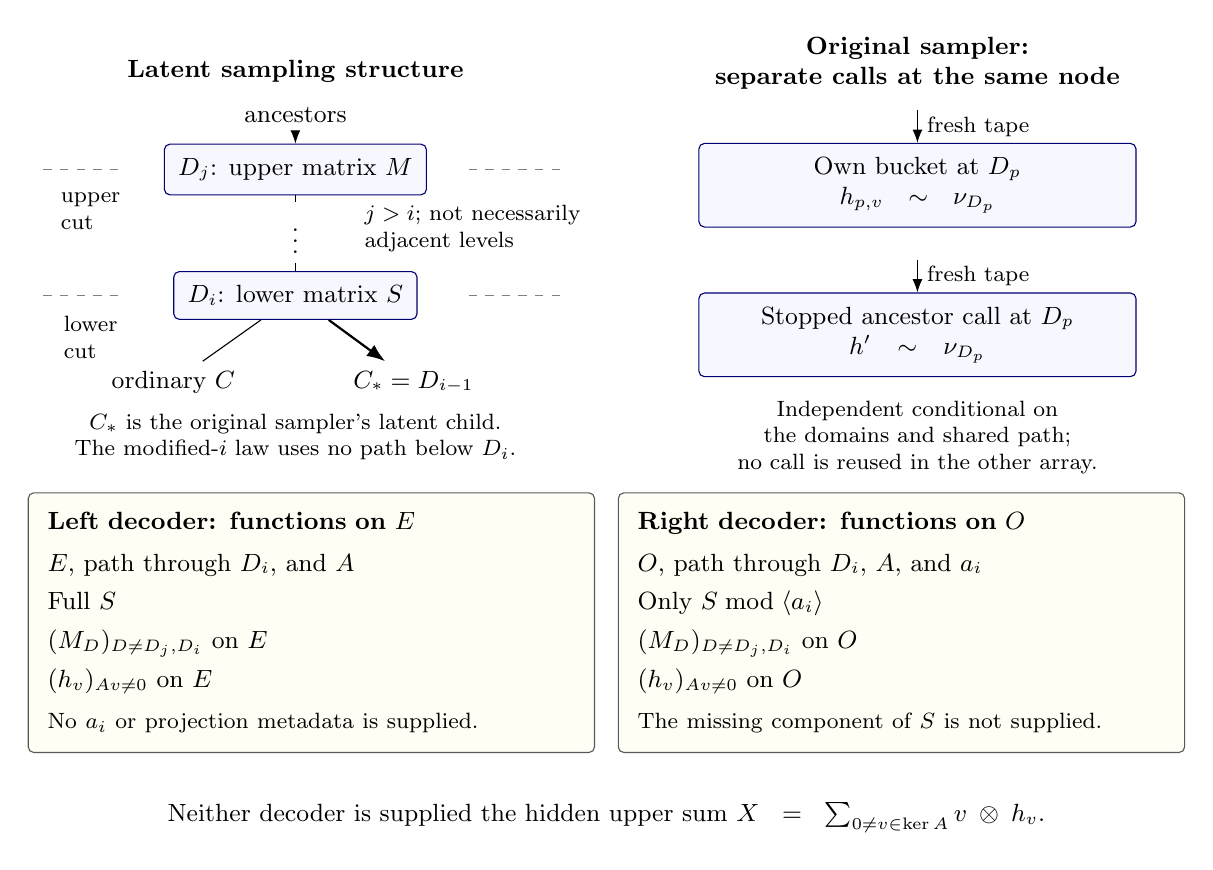
\begin{tikzpicture}[
  >=Latex, font=\small,
  cut/.style={dashed,draw=black!50},
  treebox/.style={draw=blue!45!black,rounded corners=2pt,fill=blue!3,
    align=center,inner sep=5pt},
  inputbox/.style={draw=black!65,rounded corners=2pt,fill=yellow!4,
    align=left,text width=6.7cm,inner sep=7pt}]
\node[font=\small\bfseries] at (3.2,0) {Latent sampling structure};
\node[font=\small\bfseries,align=center] at (11.1,0.1) {Original sampler:\\separate calls at the same node};
\node at (3.2,-0.55) {ancestors};
\node[treebox] (upper) at (3.2,-1.25) {$D_j$: upper matrix $M$};
\draw[->] (3.2,-0.78)--(upper);
\draw[cut] (0,-1.25)--(1.0,-1.25);
\draw[cut] (5.4,-1.25)--(6.6,-1.25);
\node[align=left,font=\footnotesize] at (0.6,-1.78) {upper\\cut};
\node[align=center] (middle) at (3.2,-2.05) {$\vdots$};
\node[align=left,font=\footnotesize] at (5.45,-2.0) {$j>i$; not necessarily\\adjacent levels};
\node[treebox] (lower) at (3.2,-2.85) {$D_i$: lower matrix $S$};
\draw (upper)--(middle);
\draw (middle)--(lower);
\draw[cut] (0,-2.85)--(1.0,-2.85);
\draw[cut] (5.4,-2.85)--(6.6,-2.85);
\node[align=left,font=\footnotesize] at (0.6,-3.38) {lower\\cut};
\node (ordinary) at (1.65,-3.95) {ordinary $C$};
\node (special) at (4.7,-3.95) {$C_* = D_{i-1}$};
\draw (lower)--(ordinary);
\draw[thick,->] (lower)--(special);
\node[align=center,text width=6.5cm,font=\footnotesize] at (3.2,-4.65)
  {$C_*$ is the original sampler's latent child.\\
   The modified-$i$ law uses no path below $D_i$.};
\node[treebox,text width=5.2cm] (own) at (11.1,-1.45)
  {Own bucket at $D_p$\\$h_{p,v}\sim\nu_{D_p}$};
\node[treebox,text width=5.2cm] (call) at (11.1,-3.35)
  {Stopped ancestor call at $D_p$\\$h'\sim\nu_{D_p}$};
\draw[->] (11.1,-0.5)--node[right,font=\footnotesize]
  {fresh tape}(own.north);
\draw[->] (11.1,-2.4)--node[right,font=\footnotesize]
  {fresh tape}(call.north);
\node[align=center,text width=5.8cm,font=\footnotesize] at (11.1,-4.65)
  {Independent conditional on the domains and shared path;\\
   no call is reused in the other array.};
\node[inputbox,anchor=north west] (left) at (-0.2,-5.35) {
  \textbf{Left decoder: functions on $E$}\\[4pt]
  $E$, path through $D_i$, and $A$\\[3pt]
  Full $S$\\[3pt]
  $(M_D)_{D\ne D_j,D_i}$ on $E$\\[3pt]
  $(h_v)_{Av\ne0}$ on $E$\\[4pt]
  \footnotesize No $a_i$ or projection metadata is supplied.
};
\node[inputbox,anchor=north east] (right) at (14.5,-5.35) {
  \textbf{Right decoder: functions on $O$}\\[4pt]
  $O$, path through $D_i$, $A$, and $a_i$\\[3pt]
  Only $S\bmod\langle a_i\rangle$\\[3pt]
  $(M_D)_{D\ne D_j,D_i}$ on $O$\\[3pt]
  $(h_v)_{Av\ne0}$ on $O$\\[4pt]
  \footnotesize The missing component of $S$ is not supplied.
};
\node[fit=(left)(right),inner sep=0pt] (cards) {};
\node[align=center,text width=14cm,below=5mm of cards.south]
  {Neither decoder is supplied the hidden upper sum
   $X=\sum_{0\ne v\in\ker A}v\otimes h_v$.};
\end{tikzpicture}
\end{document}
